% =====================================================================
%  Mechanising the Hardness of Syndrome Decoding -- CPP (acmart) version
%  Converted from the LIPIcs build (../lipics/syndrome-decoding.tex),
%  which is itself converted from ../SYNDROME_DECODING_FORMALIZATION.md.
%
%  BUILD NOTES:
%   * Engine: pdflatex. acmart ships with TeX Live.
%   * Build: pdflatex -> bibtex -> pdflatex x2 (BibTeX, ACM-Reference-Format).
%   * Submission mode: [sigplan,review,anonymous] per the CPP CFP
%     (lightweight double-blind; 12pp max excl. bibliography).
%     Camera-ready: drop review+anonymous, fill \acmConference/\acmDOI etc.
%   * Displayed Lean listings are re-wrapped BY HAND for the two-column
%     measure (~48 chars at \footnotesize tt) in faithful Lean style --
%     never introduce a soft wrap; token content must match the artifact.
%   * Unicode handling is identical to the LIPIcs build: prose via
%     newunicodechar, code via the listings literate table. Every non-ASCII
%     char inside lstinline/lstlisting MUST be in the literate table.
% =====================================================================

\documentclass[sigplan,review,anonymous]{acmart}
\settopmatter{printfolios=true,printccs=false,printacmref=false}

%% TODO CPP 2027: update from the CFP once posted (placeholders).
\acmConference[CPP '27]{Certified Programs and Proofs}{January 2027}{Mexico City, Mexico}
\acmYear{2027}
\setcopyright{none}

\usepackage{listings}
\usepackage{tikz}
\usetikzlibrary{calc}
\usepackage{newunicodechar}
\usepackage[capitalise,noabbrev]{cleveref}

% --- prose unicode -> LaTeX (pdflatex-safe) ---
\newunicodechar{≤}{\ensuremath{\le}}      \newunicodechar{≥}{\ensuremath{\ge}}
\newunicodechar{≠}{\ensuremath{\neq}}     \newunicodechar{→}{\ensuremath{\to}}
\newunicodechar{↔}{\ensuremath{\leftrightarrow}} \newunicodechar{⟺}{\ensuremath{\iff}}
\newunicodechar{⇒}{\ensuremath{\Rightarrow}} \newunicodechar{↦}{\ensuremath{\mapsto}}
\newunicodechar{∈}{\ensuremath{\in}}      \newunicodechar{∉}{\ensuremath{\notin}}
\newunicodechar{⊆}{\ensuremath{\subseteq}}\newunicodechar{⊕}{\ensuremath{\oplus}}
\newunicodechar{×}{\ensuremath{\times}}   \newunicodechar{·}{\ensuremath{\cdot}}
\newunicodechar{∘}{\ensuremath{\circ}}    \newunicodechar{∀}{\ensuremath{\forall}}
\newunicodechar{∃}{\ensuremath{\exists}}  \newunicodechar{∧}{\ensuremath{\land}}
\newunicodechar{∨}{\ensuremath{\lor}}     \newunicodechar{¬}{\ensuremath{\lnot}}
\newunicodechar{≃}{\ensuremath{\simeq}}   \newunicodechar{∞}{\ensuremath{\infty}}
\newunicodechar{∑}{\ensuremath{\sum}}     \newunicodechar{ℓ}{\ensuremath{\ell}}
\newunicodechar{σ}{\ensuremath{\sigma}}   \newunicodechar{φ}{\ensuremath{\varphi}}
\newunicodechar{τ}{\ensuremath{\tau}}     \newunicodechar{Σ}{\ensuremath{\Sigma}}
\newunicodechar{λ}{\ensuremath{\lambda}}  \newunicodechar{α}{\ensuremath{\alpha}}
\newunicodechar{β}{\ensuremath{\beta}}    \newunicodechar{μ}{\ensuremath{\mu}}
\newunicodechar{ℕ}{\ensuremath{\mathbb{N}}}
\newunicodechar{⟨}{\ensuremath{\langle}}  \newunicodechar{⟩}{\ensuremath{\rangle}}
\newunicodechar{ᵥ}{\textsubscript{v}}
\newunicodechar{₀}{\textsubscript{0}}     \newunicodechar{₁}{\textsubscript{1}}
\newunicodechar{₂}{\textsubscript{2}}     \newunicodechar{₃}{\textsubscript{3}}
\newunicodechar{ₘ}{\textsubscript{m}}     \newunicodechar{ⱼ}{\textsubscript{j}}
\newunicodechar{ᴾ}{\textsuperscript{P}}   \newunicodechar{¹}{\textsuperscript{1}}
\newunicodechar{⁻}{\textsuperscript{-}}   \newunicodechar{̄}{}% combining macron (t-bar handled in code)
\newunicodechar{ᵢ}{\textsubscript{i}}     \newunicodechar{…}{\ldots}

% --- Lean code listings style: literate unicode for pdflatex ---
\lstdefinestyle{lean}{
  basicstyle=\ttfamily\small, columns=fullflexible, keepspaces=true,
  showstringspaces=false,
  % breaklines lets \lstinline wrap at spaces (displayed blocks are wrapped by
  % hand so the wrapping shown is always faithful Lean style, never a soft wrap)
  breaklines=true, breakatwhitespace=true,
  literate=
    {t̄}{{\ensuremath{\bar{\mathtt t}}}}1
    {≤}{{$\leq$}}1 {≥}{{$\geq$}}1 {≠}{{$\neq$}}1 {→}{{$\to$}}1
    {↔}{{$\leftrightarrow$}}1 {⟺}{{$\leftrightarrow$}}1 {↦}{{$\mapsto$}}1
    {∀}{{$\forall$}}1 {∃}{{$\exists$}}1 {∧}{{$\land$}}1 {∨}{{$\lor$}}1
    {¬}{{$\lnot$}}1 {∈}{{$\in$}}1 {∉}{{$\notin$}}1 {⊆}{{$\subseteq$}}1
    {∘}{{$\circ$}}1 {⊕}{{$\oplus$}}1 {×}{{$\times$}}1 {∑}{{$\sum$}}1
    {·}{{$\cdot$}}1 {≃}{{$\simeq$}}1 {∞}{{$\infty$}}1 {ℕ}{{$\mathbb{N}$}}1
    {σ}{{$\sigma$}}1 {φ}{{$\varphi$}}1 {τ}{{$\tau$}}1 {Σ}{{$\Sigma$}}1
    {λ}{{$\lambda$}}1 {α}{{$\alpha$}}1 {β}{{$\beta$}}1 {ℓ}{{$\ell$}}1
    {⟨}{{$\langle$}}1 {⟩}{{$\rangle$}}1 {ᵥ}{{$_{\mathrm v}$}}1
    {₀}{{$_0$}}1 {₁}{{$_1$}}1 {₂}{{$_2$}}1 {₃}{{$_3$}}1
    {¹}{{$^1$}}1 {⁻}{{$^{-}$}}1 {̄}{{}}1
    {ᵢ}{{$_i$}}1 {ⱼ}{{$_j$}}1 {ₘ}{{$_m$}}1 {…}{{\ldots}}1
    {⇒}{{$\Rightarrow$}}1 {μ}{{$\mu$}}1 {ᴾ}{{$^{\mathrm P}$}}1
}
\lstset{style=lean}
% Displayed blocks drop to \footnotesize for the two-column measure.
\lstdefinestyle{leandisplay}{style=lean, basicstyle=\ttfamily\footnotesize}

% Long unbreakable code identifiers + the narrow two-column measure make some
% lines unfixable by rewording alone; let TeX loosen interword glue instead of
% overflowing into the column gutter.
\emergencystretch=2em

% =====================================================================
\title{Mechanising the Hardness of Syndrome Decoding}

%% Anonymous for review; fill for camera-ready.
\author{Anonymous Author(s)}
\affiliation{\institution{Anonymous Institution}\country{}}
\email{anon@example.org}

\ccsdesc[500]{Theory of computation~Logic and verification}
\ccsdesc[300]{Theory of computation~Problems, reductions and completeness}
\ccsdesc[300]{Security and privacy~Mathematical foundations of cryptography}

\keywords{Interactive theorem proving, Lean 4, mathlib, NP-hardness, Karp reduction,
  syndrome decoding, coding theory, 3-dimensional matching, exact cover}

\begin{document}

\begin{abstract}
The security of code-based cryptography---including McEliece-style systems, a long-standing post-quantum
reference point---rests on the conjectured intractability of \emph{syndrome decoding}: given a parity-check
matrix over GF(2), a target syndrome, and a weight bound, decide whether some error vector of bounded Hamming
weight produces that syndrome. Its NP-completeness, established by Berlekamp, McEliece, and van Tilborg in 1978,
is a textbook result; yet, to the best of our knowledge, the reduction-correctness core of that result has never
been mechanized in a proof assistant.

We present a complete, axiom-clean Lean~4 / mathlib formalization of the reduction-correctness spine of the
classical Karp chain $\textsc{3sat} \le \textsc{3dm} \le \textsc{x3c} \le$ bounded-weight GF(2) syndrome
decoding, proving each link as a \emph{both-directions} equivalence. The development mechanizes the
Garey--Johnson $\textsc{3sat} \le$ 3-dimensional-matching gadget reduction---its variable-wheel, clause, and
garbage gadgets---which is, to our knowledge, also a first in any proof assistant, together with the onward
reductions to exact-cover-by-3-sets and to syndrome decoding. Following the discipline of Kreuzer and Nipkow's
lattice-hardness formalization, we mechanize \emph{reduction correctness} and \textbf{name, rather than prove},
the surrounding complexity-theoretic apparatus---the class NP, the polynomial-time bound on the reductions, and
\textsc{3sat}'s own NP-hardness via Cook--Levin; mathlib supplies none of this scaffolding.

A central lesson is a subtlety the textbook construction glosses over: the ``obvious'' route to bounded-weight
decoding via subset-sum is \textbf{unsound over GF(2)}, where the parity check is a sum modulo~2 that discards
carries (XOR-subset-sum is in P). We route instead through a covering / odd-cover construction native to GF(2).
Every theorem depends only on Lean's three foundational axioms, build-enforced by a \texttt{\#guard\_msgs}
gate; the development---roughly 2,050 lines across eleven modules---is publicly available (anonymized for
review as supplementary material) and reproducible by \texttt{lake build}.
\end{abstract}

\maketitle

% =====================================================================
\section{Introduction}\label{sec:intro}

Code-based cryptography is among the most mature foundations for post-quantum security: McEliece-style
cryptosystems have been studied since 1978 and have remained central reference points in standardization
efforts, and their security is tied to the difficulty of decoding random-looking linear codes. The decision
form of that problem---\textbf{syndrome decoding}---asks, given a parity-check matrix $H$ over GF(2), a target
syndrome $s$, and a weight bound $w$, whether some error vector $e$ of Hamming weight at most $w$ satisfies
$H \cdot e = s$. Berlekamp, McEliece, and van Tilborg~\cite{BMvT78} proved this problem NP-complete, giving
code-based cryptography its standard worst-case complexity baseline. This is not an average-case security proof,
but it is the textbook hardness result that every account of the problem must route through.

NP-hardness reductions of this kind are the load-bearing structure of complexity theory, but they are seldom
mechanized. The Cook--Levin theorem---that SAT is NP-complete---has been formalized in Coq~\cite{GK21} and in
Isabelle/HOL~\cite{Bal23}, each building the machine model, the classes P and NP, and polynomial-time many-one
reducibility from scratch. Beyond SAT itself the mechanized landscape thins quickly: the largest collection of
formalized Karp reductions, the Isabelle \lstinline{poly-reductions} project~\cite{PolyRed}, covers SAT to
independent set, vertex cover, clique, set cover, and Hamiltonian cycle; the Coq complexity library adds
$k$SAT to clique. The classical gadget reductions to \emph{3-dimensional matching} and \emph{exact cover}, and
the reductions into \emph{coding theory}, have---to the best of our knowledge---not been mechanized at all. In
Lean~4 the situation is starker still: mathlib, the standard library, contains no notion of P, NP, SAT, or
polynomial-time reduction---its \lstinline{Computability} library provides Turing-machine models and a
stand-alone definition of polynomial-time computable functions (\lstinline{TM2ComputableInPolyTime}, whose
composition theorem is still \lstinline{proof_wanted}), but no complexity classes and no reduction framework
over them---and no coding theory beyond the Hamming metric and norm: no linear codes, syndromes, or
parity-check matrices.

This paper closes part of that gap. We give a complete, machine-checked formalization, in Lean~4 with mathlib,
of the reduction-correctness chain
\[
  \begin{gathered}
    \textsc{3sat} \;\le\; \textsc{3dm} \;\le\; \textsc{x3c} \;\le\;\\
    \text{bounded-weight GF(2) syndrome decoding,}
  \end{gathered}
\]
where \textbf{3DM} is 3-dimensional matching and \textbf{X3C} is exact-cover-by-3-sets. Each link is proved as a
\emph{both-directions} equivalence---a satisfying assignment exists iff a perfect matching exists iff an exact
cover exists iff a bounded-weight error decodes---and the chain composes to a single headline theorem relating
3-CNF satisfiability to syndrome decoding. The first link is the Garey--Johnson~\cite{GJ79} truth-setting
reduction, with its variable-wheel, clause, and garbage gadgets, which we believe is mechanized here for the
first time.

Following the discipline established by Kreuzer and Nipkow in their formalization of lattice-problem
hardness~\cite{KN23}, we are precise about what is and is not proved. We mechanize \textbf{reduction
correctness}: the many-one equivalences $\mathit{inst} \in A \iff \mathit{reduce}(\mathit{inst}) \in B$, which
are pure combinatorics and the substance of every gadget argument. We do \textbf{not} mechanize the
complexity-theoretic \emph{wrapping}: the class NP, the polynomial-time bound on the reduction functions, and
the NP-hardness of \textsc{3sat} itself (Cook--Levin). These are \emph{imported}---named explicitly as the
assumptions a hardness reading depends on, rather than smuggled into the development. mathlib offers no
complexity-theoretic scaffolding with which to formalize them. Consequently, the Lean theorem is an
unconditional reduction-correctness theorem, while the \textbf{NP-hardness label} imports the usual Cook--Levin
and polynomial-time wrapping. Any \emph{intractability} reading is further conditional on
$\mathrm P \neq \mathrm{NP}$; we make no claim about P versus NP. This is the same boundary Kreuzer and Nipkow
draw for the lattice problems, where polynomial-time-ness is ``discussed but not formalized'' and base-problem
hardness is taken as given.

Mechanization repays the effort by surfacing a subtlety the textbook construction passes over. The standard
route from exact-cover-style problems to \emph{bounded-weight decoding} runs through subset-sum; but
\textbf{subset-sum is the wrong target over GF(2)}, where the parity check $H \cdot e$ is a sum modulo~2 and the
carries that make integer subset-sum hard are discarded---XOR-subset-sum is solvable in polynomial time by
Gaussian elimination. We route instead through a \emph{covering} (odd-cover) construction native to GF(2), in
which the syndrome's parity bits encode an exact cover directly. Recognizing and repairing this mismatch---
invisible at the level of an informal ``and now reduce to decoding''---is, in the spirit of~\cite{KN23}, a
contribution of the formalization itself.

Our contributions are:
\begin{itemize}
  \item \textbf{(C1)} To the best of our knowledge, the \textbf{first machine-checked reduction-correctness
    spine for the NP-hardness of bounded-weight GF(2) syndrome decoding} in any proof assistant---the decision
    problem shown NP-complete by~\cite{BMvT78}, with the NP / polynomial-time wrapping imported as stated above.
  \item \textbf{(C2)} To our knowledge, the \textbf{first mechanization of the Garey--Johnson
    $\textsc{3sat} \le \textsc{3dm}$ gadget reduction and of $\textsc{3dm} \le \textsc{x3c}$} in any proof
    assistant.
  \item \textbf{(C3)} A \textbf{GF(2)-native exact-cover-to-decoding reduction}, and the identification and
    repair of the subset-sum-over-GF(2) pitfall.
  \item \textbf{(C4)} The chain delivered as a single, axiom-clean Lean~4 / mathlib artifact
    ($\approx$2{,}050 lines, eleven modules) with axiom-cleanliness build-enforced by a \lstinline{#guard_msgs}
    gate---introducing the parity-check / syndrome / bounded-weight-decoding decision vocabulary into Lean, an
    ecosystem with no prior coding-theory \emph{hardness} formalization.
  \item \textbf{(C5)} An \textbf{experience report} on the \emph{name-the-imported-wall} discipline, the
    proof-engineering walls we met, and a brief account of the AI-assisted workflow used to build the
    development.
\end{itemize}

The full development is available (anonymized for review) as supplementary material and is reproducible by
\lstinline{lake build}; every headline theorem's axiom footprint is pinned by a \lstinline{#guard_msgs} gate, so
a \lstinline{sorry}, a \lstinline{native_decide}, or any stray axiom fails the build. \Cref{sec:bg} fixes the
four problems and the Lean/mathlib setting. \Cref{sec:chain} develops the reduction chain. \Cref{sec:gf2}
presents the GF(2)-native decoding reduction and what the development imports. \Cref{sec:eng} is the engineering
and experience report. \Cref{sec:app} relates the result to its motivating application. \Cref{sec:related}
surveys related work and \Cref{sec:concl} concludes.

% =====================================================================
\section{Background}\label{sec:bg}

\subsection{The four decision problems}\label{sec:problems}

\paragraph{3SAT} A 3-CNF formula over $n$ Boolean variables and $m$ clauses, each clause an ordered triple of
literals; \lstinline{Satisfiable φ} holds when some assignment satisfies every clause. We represent a literal
as a variable index with a sign (\lstinline{Fin n × Bool}), a clause as \lstinline{Fin 3 → Literal}, and a
formula as \lstinline{Fin m → Clause}.

\paragraph{3-Dimensional Matching (3DM)} Given a family of triples over three ground sets $W, X, Y$, a
\emph{perfect matching} is a selection covering each element of each ground set exactly once.

\paragraph{Exact Cover by 3-Sets (X3C)} Given a family \lstinline{c : Fin s → Finset X} of 3-element subsets
of a ground set $X$, an \emph{exact cover} is a selection covering each point exactly once.

\paragraph{Bounded-weight syndrome decoding} Given a parity-check matrix $H$ over GF(2), a syndrome, and a
weight bound $q$, decide whether some error $e$ of Hamming weight $\le q$ satisfies $H \cdot e = s$. This is the
decision form of minimum-distance decoding---the problem~\cite{BMvT78} showed NP-complete.

\subsection{The classical reductions}\label{sec:classical}

The chain composes three classical many-one reductions. \textbf{(1)} The Garey--Johnson~\cite{GJ79}
\emph{truth-setting} reduction $\textsc{3sat} \le \textsc{3dm}$ encodes each variable as a ``wheel'' gadget
admitting exactly two matchings (its two truth values), each clause as a gadget coverable iff one of its
literals is true, with \emph{garbage} elements absorbing unused gadget tips. \textbf{(2)}
$\textsc{3dm} \le \textsc{x3c}$ is a relabelling: a triple $(w,x,y)$ becomes the 3-set $\{w,x,y\}$ over the
disjoint union $W \oplus X \oplus Y$. \textbf{(3)} $\textsc{x3c} \le$ bounded-weight GF(2) decoding takes the
incidence matrix of the set family as the parity check and the all-ones vector as the syndrome
(\Cref{sec:gf2}).

\subsection{Lean 4, mathlib, and axiom-cleanliness}\label{sec:axiomclean}

We work in Lean~4 with mathlib v4.30.0. A Lean proof is trusted exactly insofar as one trusts the kernel and
the axioms a result invokes; mathlib's developments rest on three foundational axioms---\lstinline{propext},
\lstinline{Classical.choice}, \lstinline{Quot.sound}. We call a result \emph{axiom-clean} when
\lstinline{#print axioms} reports only these (or a subset), with no \lstinline{sorryAx} (which a
\lstinline{sorry} introduces) and no \lstinline{Lean.ofReduceBool} (which \lstinline{native_decide} introduces,
trusting the compiler's evaluator); kernel \lstinline{decide} is axiom-clean. mathlib supplies finite types,
\lstinline{Finset}s, matrices over \lstinline{ZMod 2}, and the Hamming norm---but no complexity theory and no
coding theory beyond the Hamming metric.

% =====================================================================
\section{The Reduction Chain}\label{sec:chain}

The chain is built bottom-up across nine modules, landing on the X3C and decoding endpoints. We describe the
$\textsc{3sat} \le \textsc{3dm}$ reduction---the substantive part---and then the composition.

\subsection{Encoding 3SAT}\label{sec:3sat}

The 3SAT definitions are standard combinatorics over finite types, so satisfiability is decidable on concrete
instances. We lock the encoding \emph{before} the gadgets depend on it with two kernel-\lstinline{decide}-
validated examples---a satisfiable and an unsatisfiable formula---exercising both literal signs.

\subsection{The variable-wheel gadget}\label{sec:wheel}

A variable's wheel of size $m$ owns, per spoke \lstinline{j : Fin m}, two internal nodes \lstinline{a j},
\lstinline{b j} and two tips, with a positive triple \lstinline{t_j = (posTip j, a j, b j)} and a negative
triple \lstinline{t̄_j = (negTip j, a (j+1), b j)}, where \lstinline{j+1} is cyclic in \lstinline{Fin m}. Since
\lstinline{b j} lies only in \lstinline|{t_j, t̄_j}|, any internal cover selects one triple per spoke---a
\lstinline{Selection σ : Fin m → Bool}. Node \lstinline{a j} is covered exactly once iff exactly one of
$\{\sigma\,j = \mathtt{true},\ \sigma\,(j{-}1) = \mathtt{false}\}$ holds; by the Boolean identity
$\mathtt{xor}\ a\ (\lnot b) = (a = b)$, that collapses to $\sigma\,j = \sigma\,(j{-}1)$. The engine of the
gadget is then:
\begin{lstlisting}[style=leandisplay]
theorem validCover_iff_const (hm : 0 < m)
    (σ : Selection m) :
    ValidCover σ ↔
      (σ = fun _ => true) ∨ (σ = fun _ => false)
\end{lstlisting}
A valid internal cover is \emph{constant}---and the two constants are the variable's two truth values. The
forward direction is a strong induction showing a cyclic equal-neighbour selection is constant. Geometrically
(\Cref{fig:wheel}) the gadget \emph{is} the even cycle $C_{2m}$: its $2m$ internal nodes are the cycle
vertices, its $2m$ triples the cycle edges, and a valid internal cover is a perfect matching of that
cycle---of which an even cycle has exactly two.

\begin{figure*}[t]
\centering
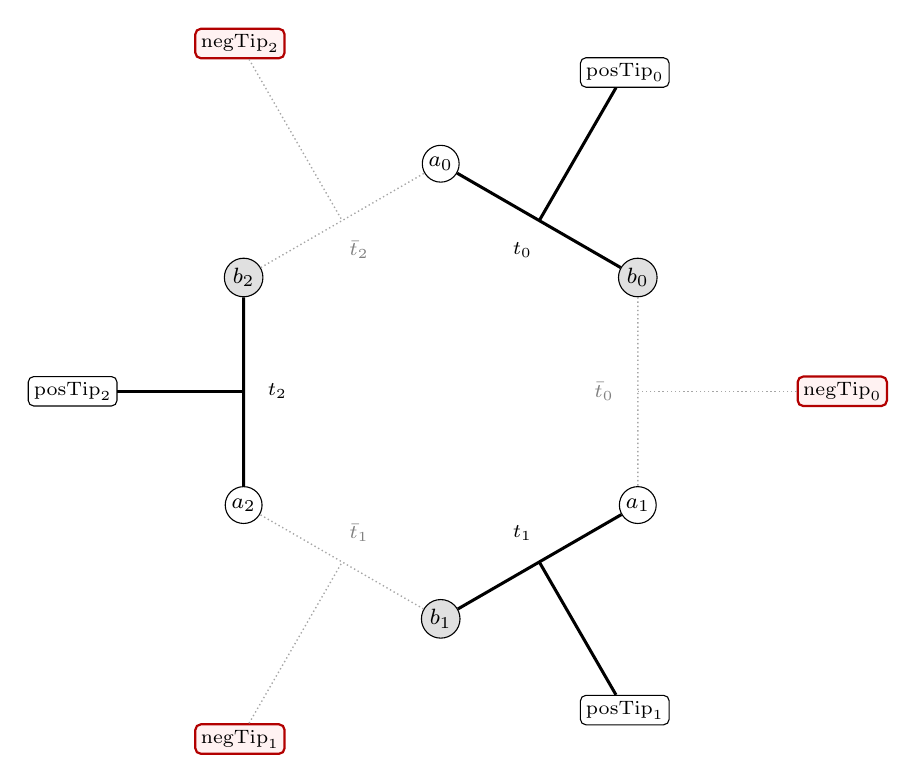
\begin{tikzpicture}[scale=1.7,
    anode/.style={circle, draw, fill=white, inner sep=1.3pt, font=\footnotesize},
    bnode/.style={circle, draw, fill=black!12, inner sep=1.3pt, font=\footnotesize},
    tip/.style={rounded corners=2pt, draw, fill=white, inner sep=2pt, font=\scriptsize},
    freetip/.style={rounded corners=2pt, draw=red!70!black, thick, fill=red!5,
                    inner sep=2pt, font=\scriptsize},
    sel/.style={line width=1.1pt},
    unsel/.style={gray!70, line width=0.5pt, densely dotted}]
  \node[anode] (a0) at (90:1.7)  {$a_0$};   \node[bnode] (b0) at (30:1.7)  {$b_0$};
  \node[anode] (a1) at (-30:1.7) {$a_1$};   \node[bnode] (b1) at (-90:1.7) {$b_1$};
  \node[anode] (a2) at (-150:1.7){$a_2$};   \node[bnode] (b2) at (150:1.7) {$b_2$};
  \draw[sel] (a0)--(b0); \draw[sel] (a1)--(b1); \draw[sel] (a2)--(b2);
  \draw[unsel] (b0)--(a1); \draw[unsel] (b1)--(a2); \draw[unsel] (b2)--(a0);
  \node[tip] (p0) at (60:2.75) {$\mathrm{posTip}_0$};
  \node[tip] (p1) at (-60:2.75){$\mathrm{posTip}_1$};
  \node[tip] (p2) at (180:2.75){$\mathrm{posTip}_2$};
  \draw[sel] (p0)--($(a0)!.5!(b0)$); \draw[sel] (p1)--($(a1)!.5!(b1)$);
  \draw[sel] (p2)--($(a2)!.5!(b2)$);
  \node[freetip] (q0) at (0:3.0)    {$\mathrm{negTip}_0$};
  \node[freetip] (q1) at (-120:3.0) {$\mathrm{negTip}_1$};
  \node[freetip] (q2) at (120:3.0)  {$\mathrm{negTip}_2$};
  \draw[unsel] (q0)--($(b0)!.5!(a1)$); \draw[unsel] (q1)--($(b1)!.5!(a2)$);
  \draw[unsel] (q2)--($(b2)!.5!(a0)$);
  \node[font=\scriptsize] at (60:1.22)  {$t_0$}; \node[font=\scriptsize] at (-60:1.22){$t_1$};
  \node[font=\scriptsize] at (180:1.22) {$t_2$};
  \node[font=\scriptsize,gray] at (0:1.22)   {$\bar t_0$};
  \node[font=\scriptsize,gray] at (-120:1.22){$\bar t_1$};
  \node[font=\scriptsize,gray] at (120:1.22) {$\bar t_2$};
\end{tikzpicture}
\caption{The variable-wheel gadget for $m=3$ (general $m$: the even cycle $C_{2m}$). Internal nodes $a_j$
(open) and $b_j$ (shaded) alternate around the ring; each ring edge is a triple carrying a tip. The positive
triple $t_j=(\mathrm{posTip}_j,a_j,b_j)$ and the negative $\bar t_j=(\mathrm{negTip}_j,a_{j+1},b_j)$ share
$b_j$, so any internal cover selects exactly one per spoke (a \emph{Selection} $\sigma$); the $a$-node
sharing---$t_j$ contributes $a_j$ while $\bar t_{j-1}$ contributes $a_{(j-1)+1}=a_j$---then forces $\sigma$ to
be constant, i.e.\ one of the cycle's exactly two perfect matchings, the variable's two truth values. The
selected matching (bold, all $t_j$) covers every internal node once, consumes the positive tips, and
\emph{frees} the negative tips (boxed) for the clause gadgets; the other matching (dotted, all $\bar t_j$) does
the reverse. The negative triple's $a$-node is the cyclic successor $a_{j+1}$---the $+1$ shift responsible for
the $a$-/$b$-node asymmetry in the incidence lemmas (\Cref{sec:assembly}).}
\label{fig:wheel}
\end{figure*}

\subsection{The clause gadget and the polarity bridge}\label{sec:clause}

The clause gadget's internal pair is coverable iff some literal's tip is free (\lstinline{clauseCoverable}).
The \emph{polarity bridge} connects the wheel's raw free-tip predicate---under the convention that a variable
assigned \lstinline{aᵢ} runs the constant selection \lstinline{fun _ => ¬aᵢ}---to literal evaluation:
\begin{lstlisting}[style=leandisplay]
theorem litTipFree_iff_eval (a : Assignment n)
    (l : Literal n) {m : ℕ} [NeZero m]
    (j : Fin m) :
    litTipFree a l j ↔ evalLiteral a l = true
\end{lstlisting}
A tip is free exactly when its literal is true. This discharges the truth-value labelling and is the one place
a sign error would silently corrupt the reduction; we additionally lock it with a four-case
$(\mathit{sign} \times a_i)$ \lstinline{decide}.

\subsection{Global assembly}\label{sec:assembly}

The three coordinate sets are the tips \lstinline{Tip = Fin n × Fin m × Bool} (the $W$-part) and
\lstinline{XNode = YNode}, the disjoint sum \lstinline{(Fin n × Fin m) ⊕ Fin m ⊕ Fin (m·(n-1))} of
variable-internal nodes, clause-internal nodes, and garbage. Each has cardinality $2mn$; the garbage count
$m(n{-}1)$ is exactly what balances the books, and the equality $n m + m + m(n{-}1) = 2mn$ requires $n \ge 1$.
A triple family \lstinline{tripleFn} emits each gadget triple, and \lstinline{reduce φ} re-indexes it along the
canonical finite equivalence into the \lstinline{Fin s → W×X×Y} shape the matching problem expects.
Cardinality lemmas feed \lstinline{reduce_chain_connects}, wiring \lstinline{reduce φ} onto the
already-formalized $\textsc{3dm} \le \textsc{x3c} \le$ decoding tail.

To keep the heavy counting over the structured sum-type index rather than an opaque \lstinline{Fin s}, we prove
a generic reindexing bridge \lstinline{ThreeDM_I t ↔ ThreeDM (t ∘ e.symm)} (along
\lstinline{e := Fintype.equivFin _}) and carry the gadget arguments over the natural index. Six \emph{incidence}
lemmas then characterize which triple-indices cover each node. The subtle one is a cyclic-shift asymmetry: an
$a$-node \lstinline{inl(i,j)} is covered by \lstinline{posT(i,j)} and \lstinline{negT(i, j-1)}, whereas a
$b$-node is covered by \lstinline{posT(i,j)} and \lstinline{negT(i,j)}---no shift. A wrong shift here corrupts
the wheel-state extraction downstream.

\subsection{Forward and reverse correctness}\label{sec:fwdrev}

The \textbf{reverse} direction reads an assignment out of a matching: the $b$-node and $a$-node ``covered
exactly once'' facts force each wheel's \lstinline{Selection} to be a \lstinline{ValidCover}, hence constant by
the engine (giving each \lstinline{aᵢ}); each clause's selected slot's tip is forced free, hence its literal
true.

The \textbf{forward} direction \emph{builds} the matching from a satisfying assignment: the constant wheel cover
per variable, one satisfied-slot triple per clause, and the leftover free tips absorbed by a counted
\emph{garbage bijection}---\lstinline{Fintype.equivFinOfCardEq} on the size-$m(n{-}1)$ set of unclaimed free
tips. The three cover conditions split over the disjoint summands, and the tip count is a three-way partition
(consumed / free-and-claimed / free-and-unclaimed), each summing to one.

The forward/reverse asymmetry is striking---\lstinline{reverse} is 184 lines, \lstinline{forward} 543:
constructing and counting a perfect matching, garbage bijection included, is materially harder than reading an
assignment out of a given one.

\subsection{Composition}\label{sec:compose}

Both directions are packaged as \lstinline{sat_iff_threeDM_I}, the pair \lstinline{⟨forward φ, reverse φ⟩};
transported through the reindexing bridge to the real \lstinline{Fin s}-indexed \lstinline{ThreeDM}, then
through \lstinline{reduce_chain_connects}, this yields the headline:
\begin{lstlisting}[style=leandisplay]
theorem sat_iff_decodes (φ : Formula n m) :
    Satisfiable φ ↔
      DecodingNPHard.Decodes
        (reduce3DM (reduce φ)) (2 * m * n)
\end{lstlisting}
$\textsc{3sat} \le \textsc{3dm} \le \textsc{x3c} \le$ decoding, closed end to end. (The
$\textsc{3dm} \le \textsc{x3c}$ and $\textsc{x3c} \le$ decoding endpoints, \Cref{sec:gf2}, supply the tail.)

% =====================================================================
\section{The GF(2)-Native Decoding Reduction and the Imported Wall}\label{sec:gf2}

\subsection{The subset-sum trap over GF(2)}\label{sec:trap}

One might expect the route from a covering problem to bounded-weight decoding to pass through subset-sum:
encode memberships as integers, ask for a low-weight subset summing to a target. \textbf{Over GF(2) this is
unsound.} The parity check $H \cdot e$ is a sum modulo~2---the carries that make integer subset-sum NP-hard are
discarded, and XOR-subset-sum is solvable in polynomial time by Gaussian elimination. The correct source
structure is \emph{covering}, where mod-2 addition is the native operation. (The development records this as the
reduction's failure mode: a wrong source problem yields a wrong reduction.)

\subsection{The covering reduction}\label{sec:covering}

An X3C instance \lstinline{c : Fin s → Finset X} becomes the parity-check matrix whose column $i$ is the GF(2)
indicator of the 3-set \lstinline{c i}, with the all-ones syndrome:
\begin{lstlisting}[style=leandisplay]
def Hmat : Matrix X (Fin s) (ZMod 2) :=
  Matrix.of (fun x i => if x ∈ c i then 1 else 0)
def Decodes : Prop :=
  ∃ e : Fin s → ZMod 2,
    Hmat c *ᵥ e = allOnes c ∧ hammingNorm e ≤ q
\end{lstlisting}
The connection lemma makes the encoding exact: for the 0/1 indicator \lstinline{eOf T} of a selection $T$, the
syndrome coordinate at point $x$ is the mod-2 cast of its cover count,
\begin{lstlisting}[style=leandisplay]
theorem syndrome_eq_coverCount_cast
    (T : Finset (Fin s)) (x : X) :
    (Hmat c *ᵥ eOf c T) x
      = ((coverCount c T x : ℕ) : ZMod 2)
\end{lstlisting}
so ``syndrome $=$ all-ones'' says exactly ``every point is covered an \emph{odd} number of times''. An exact
cover (count one) is odd; conversely a weight-$q$ odd cover must be exact, because the weight bound
$q = |X|/3$ and the 3-uniformity, via the double-count $\sum_x \mathit{coverCount} = 3 \cdot |T|$, pin
$|T| = q$ and then force every count to one. Both directions are machine-checked (the iff carries the
structural hypotheses the prose uses---that every set has three elements and that $|X| = 3q$):
\begin{lstlisting}[style=leandisplay]
theorem reduction_iff
    (hc : ∀ i, (c i).card = 3)
    (hX : Fintype.card X = 3 * q) :
    X3C c ↔ Decodes c q
\end{lstlisting}
At the chain's head these hypotheses are discharged by the reduction's own cardinality lemmas, so
\lstinline{sat_iff_decodes} is unconditional (modulo $n, m \ge 1$). The landed \lstinline{Decodes} is precisely
the decision form of the minimum-coset-weight quantity whose hardness a syndrome certificate's soundness
assumes (\Cref{sec:app}).

\subsection{Naming the imported wall}\label{sec:wall}

What we do \emph{not} prove is the complexity-theoretic wrapping. The reduction functions are visibly local---
each gadget index maps to one triple, each triple to one 3-set, each 3-set to one matrix column---but
``polynomial-time'' is unformalized: mathlib's lone polynomial-time notion
(\lstinline{TM2ComputableInPolyTime}) is a stand-alone definition, its composition theorem still
\lstinline{proof_wanted}, with no reduction framework built on it. NP membership, and \textsc{3sat}'s own
NP-hardness (Cook--Levin), are likewise imported. We name this boundary in the development: a
\lstinline{CertWall} module \emph{types} the imported quantity, and every module's documentation states the
limit. The Lean output is therefore an \emph{unconditional reduction-correctness theorem}; the NP-hardness
reading attaches the imported wrapping (Cook--Levin and the poly-time bound), and only an intractability reading
further assumes $\mathrm P \neq \mathrm{NP}$.

% =====================================================================
\section{Engineering and Experience Report}\label{sec:eng}

\subsection{Axiom-cleanliness as a build invariant}\label{sec:gate}

Every headline theorem is axiom-clean. We make this \emph{self-checking}: an \lstinline{AxiomAudit} module pins
each result's \lstinline{#print axioms} output with \lstinline{#guard_msgs}, so a regression---a stray
\lstinline{sorry}, a \lstinline{native_decide}, any extra axiom---changes the captured message and fails
\lstinline{lake build}. The referee-free promise can no longer silently regress.

The pattern is small and project-agnostic: one audit module imports every load-bearing module and pins one
\lstinline{#guard_msgs in #print axioms} block per exported theorem; extending the gate is one block per new
result, and guarding the top-level \lstinline{sat_iff_decodes} transitively protects the whole chain (its axiom
set would change if any dependency's did). Before the gate, axiom-cleanliness was checked by a human reading
\lstinline{#print axioms} output; now the kernel's own output is the regression test, with no CI scripting
outside the build. One practical subtlety: \lstinline{#guard_msgs} captures \emph{every} message the command
emits, so the gate interacts with active linters---under a full \lstinline{lake build} the mathlib whitespace
linter also fires, and each \lstinline{#print axioms} must sit on its own line at column~0, or the linter's
message lands in the captured text and spuriously fails the gate.

\subsection{Proof-engineering walls}\label{sec:walls}

Mechanizing the chain met several walls worth recording.
\begin{itemize}
  \item \textbf{Decidable equality on a four-way sum.} The triple-index type is a four-way nested
    \lstinline{Sum} of products; inside large proof contexts (where the filter-rewrites force the search),
    \lstinline{DecidableEq} synthesis exceeds the default \lstinline{synthInstance.maxSize}. A scoped
    \lstinline{set_option synthInstance.maxSize 512} clears it.
  \item \textbf{Rewriting a filter predicate.} Rewriting the predicate of a \lstinline{Finset.filter} through
    an incidence lemma fails directly---\lstinline{DecidablePred} cannot be synthesized at the rewrite
    site---so we name the rewritten Finset in an explicit
    \lstinline{have heq := Finset.filter_congr …; rw [heq]}, forcing elaboration with the instance in scope.
  \item \textbf{The garbage bijection.} The forward construction needs a bijection from the index set
    \lstinline{Fin (m(n-1))} onto the assignment-dependent set of unclaimed free tips; its existence follows
    from a cardinality equality supplied non-constructively by \lstinline{Fintype.equivFinOfCardEq}, and the
    counting ($|\mathit{free}| = mn$, $|\mathit{claimed}| = m$, $|\mathit{unclaimed}| = m(n{-}1)$) is the real
    work.
  \item \textbf{Cyclic \lstinline{Fin} arithmetic.} The wheel's cyclic predecessor uses \lstinline{Fin m}'s
    additive-group structure under \lstinline{[NeZero m]}; the defining $j{+}1 = j_0 \iff j = j_0{-}1$ is
    \lstinline{eq_sub_iff_add_eq}.
\end{itemize}

\subsection{The development at a glance}\label{sec:metrics}

The chain is roughly 2,050 lines across eleven modules (1,638 in the nine new reduction modules; the X3C and
decoding endpoints supply the remainder), comprising on the order of fifty theorems and lemmas. Every headline
result depends only on \lstinline{propext}, \lstinline{Classical.choice}, and \lstinline{Quot.sound} (or a
subset), and the development rebuilds via \lstinline{lake build} atop a cached mathlib, reproducible from the
artifact.

The artifact is the development itself: from a clean checkout, \lstinline{lake exe cache get} followed by
\lstinline{lake build} re-elaborates every proof and re-runs the axiom gate atop the cached mathlib, in minutes
on commodity hardware; we re-verified exactly this flow from a fresh clone for this submission. There is
nothing else to trust: no vendored binaries, no extracted code, no \lstinline{native_decide}---the trusted base
is the Lean kernel, the three foundational axioms, and the pinned toolchain (Lean and mathlib v4.30.0).

\subsection{What ports out of this development}\label{sec:portable}

Three pieces of this development are reduction-agnostic.

\paragraph{The reindexing bridge} Decision problems are conventionally stated over an opaque index
(\lstinline{Fin s → W×X×Y}), but gadget arguments live over structured indexes---here, a four-way sum of
products. The generic bridge \lstinline{ThreeDM_I t ↔ ThreeDM (t ∘ e.symm)} (along
\lstinline{e := Fintype.equivFin _}) lets the entire correctness proof run over the natural index and
transports the result to the opaque statement at the end. Any mechanized gadget reduction whose instance space
has structure---which is to say, any gadget reduction---needs exactly this bridge, and it is independent of
3DM.

\paragraph{The counted-bijection pattern} Gadget constructions routinely end with ``absorb the leftovers with
garbage''---an informal step that, mechanized, becomes: partition the resource (here, tips) into consumed /
claimed / unclaimed classes, prove the three cardinalities, and obtain the absorbing bijection
non-constructively from \lstinline{Fintype.equivFinOfCardEq}. The shape (three-way partition count, then a
counted bijection) is the reusable unit; the 543-line forward proof is mostly instances of it.

\paragraph{The encoding lock} Before any gadget depends on the 3SAT encoding, two kernel-\lstinline{decide}
examples (one satisfiable, one unsatisfiable, exercising both literal signs) pin its semantics; the polarity
bridge is additionally locked by a four-case $(\mathit{sign} \times a_i)$ \lstinline{decide}. Locking an
encoding with decidable concrete instances \emph{before} building on it is cheap insurance against the silent
sign error---the class of bug a reduction cannot recover from---and costs the kernel milliseconds.

\subsection{A note on the workflow}\label{sec:workflow}

The development was produced with substantial AI assistance, under a fixed discipline: each module was scoped
and reconnoitred against the live toolchain, drafted, adversarially reviewed for correctness and over-claim,
then reproduced independently by the author before commit. The axiom-clean \lstinline{#guard_msgs} gate and the
kernel re-check make this provenance immaterial to the result's \emph{validity}---the kernel certifies the
proofs however they were written---but we record it honestly as how the development was built.

% =====================================================================
\section{The Certificate Application}\label{sec:app}

Bounded-weight GF(2) syndrome decoding is not an arbitrary target: it is the hardness assumption beneath
code-based cryptography. McEliece-style cryptosystems encrypt by adding a bounded-weight error to a codeword,
and their security is tied to the difficulty of decoding. Our chain machine-checks that this decoding problem is
reduction-equivalent to a canonical NP-hard problem, anchoring the qualitative ``decoding is hard'' intuition to
\textsc{3sat}, and the landed \lstinline{Decodes} instance is exactly the decision form of the
minimum-coset-weight quantity a syndrome certificate's soundness rests on---so the development connects, in one
formal artifact, that certificate's imported hardness wall to the canonical NP-hard problem.

The wall is typed, not only named. The artifact's \lstinline{CertWall} module defines the semantic quantity
behind the certificate---\lstinline{minCosetWeight}, the least Hamming weight over a syndrome's coset, whose
bounded decision form is exactly the \lstinline{Decodes} our chain lands on---and proves the \emph{shape} of
the import from the consumer's side. The true quantity is a code invariant: a change of parity-check basis
(left-multiplication by an invertible matrix) leaves it unchanged (\lstinline{minCosetWeight_rowEquiv}). The
verifier's cheap sound bound provably is not: on two bases of the \emph{same} code it returns the true distance
on one and collapses to zero on the other (\lstinline{colWeightLb_not_basis_invariant}, a witnessed
counterexample). And a conditional theorem (\lstinline{tight_bound_decodes}) types the closing observation: a
cheap bound that is \emph{tight} on a syndrome computes the decoding distance there. Jointly: a cheap,
basis-robust, tight bound would \emph{be} a decoder, so the cheap bound's basis-dependence is the visible edge
of the imported hardness---now machine-checked on both sides, anchored below by this paper's chain (decoding is
at least as hard as \textsc{3sat}, modulo the named wrapping) and bounded above by the typed conditional
(anything that closed the gap would discharge the import). No hardness is proved on either side; what is
kernel-checked is where the assumption lives.

We are careful about the boundary.~\cite{BMvT78} worst-case NP-hardness is the standard complexity baseline
every account of the problem routes through, but it is \textbf{not an average-case security proof}: McEliece's
security rests on the average-case hardness of decoding \emph{random} codes---a strictly stronger assumption
that worst-case NP-hardness does not establish. Our contribution puts the worst-case baseline---its
reduction-correctness spine---on a machine-checked footing; it does not certify the cryptographic assumption,
and we claim no such thing.

% =====================================================================
\section{Related Work}\label{sec:related}

\paragraph{Cook--Levin and the complexity wrapping} The foundational result we import---that SAT is
NP-hard---has two from-scratch mechanizations. Gäher and Kunze~\cite{GK21} formalized the Cook--Levin theorem in
Coq over the weak call-by-value $\lambda$-calculus $L$, building the classes P and NP, polynomial-time many-one
(Karp) reductions, and NP-completeness, as part of the Coq Library of Complexity Theory atop the Coq Library of
Undecidability Proofs~\cite{CLUP}. Balbach~\cite{Bal23} gave an Isabelle/HOL formalization over deterministic
multi-tape Turing machines, proving SAT NP-hard via an oblivious verifier and emphasizing that both the
complexity-theoretic concepts and the polynomiality of the reduction use the \emph{same} model of computation.
Our development depends on exactly this result and treats it as the terminal imported wall; neither
formalization addresses 3DM, X3C, or decoding.

\paragraph{Mechanized Karp reductions} Downstream of SAT, the Isabelle \lstinline{poly-reductions}
project~\cite{PolyRed} formalizes, with explicit polynomial running-time bounds, a family of
reductions---3CNF-SAT to independent set, vertex cover, clique, and set cover, together with
Hamiltonian-cycle variants and vertex cover to feedback node set---going beyond reduction correctness to
\emph{poly-time} reductions. The Coq complexity library contributes $k$SAT to clique. None of these touches
3-dimensional matching, exact cover, subset-sum, or any coding problem; the gadget reductions we mechanize are
disjoint from this corpus. As of~\cite{GK21} (2021), the downstream Karp reductions---including 3DM and exact
cover---were listed explicitly as enabled-but-not-yet-undertaken future work.

\paragraph{Lattice hardness---the methodological precedent} Closest in genre is Kreuzer and
Nipkow's~\cite{KN23} Isabelle/HOL verification of NP-hardness reduction functions for the exact lattice problems
CVP and SVP (in the $\ell_\infty$ norm), via reductions from subset-sum and partition. The scope matches ours
almost exactly: they verify reduction correctness, take the base problems' NP-hardness \emph{as given}, and
explicitly discuss---but do not formalize---polynomial-time-ness (their \S7). Notably, their formalization
\emph{uncovered gaps in the textbook proofs} it mechanized, lending the experience report a contribution
independent of the underlying mathematics. CVP is the lattice analogue of nearest-codeword decoding, making
this work \emph{coding-adjacent}; but it is a distinct problem domain over a different algebraic structure, it
does not subsume the syndrome-decoding result, and we adopt its honest experience-report framing rather than
competing with it.

\paragraph{Formalized coding theory} The most developed formalized coding theory in any assistant is the
Coq/MathComp \lstinline{infotheo} library~\cite{AGS20}, which formalizes linear error-correcting codes and
Hamming, Reed--Solomon, BCH, Reed--Muller, and cyclic codes, with LDPC sum-product decoding and an extracted
verified decoder, alongside Shannon's theorems. Crucially, this is decoding-\emph{algorithm correctness}, not
decoding-\emph{hardness}: \lstinline{infotheo} proves that decoders compute correctly, not that decoding is
hard---the two are orthogonal, and only the latter is our subject. In Lean, mathlib~\cite{mathlib} provides only
the Hamming metric and norm (\lstinline{InformationTheory.Hamming}); a search of mathlib for parity-check,
syndrome, generator, or linear-code primitives returns nothing. External Lean coding-theory work is likewise
correctness-oriented: the early Cotoleta library formalized repetition and Hamming(7,4) codes~\cite{HNK16}, the
ArkLib SNARK-verification effort is building Reed--Solomon proximity infrastructure~\cite{ArkLib}, and---nearest
our subject---Lean-QEC provides a stabilizer-code and verified distance-certificate
pipeline~\cite{ELWT26}. Lean-QEC runs the \emph{converse} direction to ours: it reduces a
code-\emph{distance} condition \emph{to} SAT for verification (observing that distance certification is NP-hard
in general, without proving it), rather than reducing SAT \emph{to} a coding problem to mechanize hardness; it
contains no Garey--Johnson gadget reduction and no syndrome-decoding hardness result. Our development therefore
contributes, to our knowledge, the first machine-checked reduction-correctness spine for bounded-weight GF(2)
syndrome-decoding hardness and introduces that decision problem into a Lean setting.

\paragraph{The gap} No prior work mechanizes the hardness of syndrome decoding, the Garey--Johnson
$\textsc{3sat} \le \textsc{3dm}$ reduction, or $\textsc{3dm} \le \textsc{x3c}$, in any system. Lean's
complexity-theory ecosystem is young but no longer empty: a substantial Lean~4 development~\cite{Sim26}
mechanizes coNP-, $\Sigma_2^{\mathrm P}$-, PP-, and PSPACE-completeness results (with their reductions) for a
``physical counting'' problem family, so we claim no \emph{first complexity reduction in Lean}---our first-ness
is specific to the coding-theory hardness and the classical $\textsc{3sat} \le \textsc{3dm} \le \textsc{x3c}$
gadget chain, which neither~\cite{Sim26} nor~\cite{ELWT26} nor any other community effort touches. We will
re-survey immediately before submission.

% =====================================================================
\section{Conclusion and Future Work}\label{sec:concl}

We have given a complete, axiom-clean Lean~4 / mathlib formalization of the reduction-correctness spine of the
chain $\textsc{3sat} \le \textsc{3dm} \le \textsc{x3c} \le$ bounded-weight GF(2) syndrome decoding. Both
directions of each link are machine-checked; the reduction-correctness spine for the Garey--Johnson
truth-setting chain and for bounded-weight GF(2) syndrome-decoding hardness is, to the best of our knowledge,
mechanized here for the first time in any proof assistant. The development brings this coding-theoretic hardness
problem---in the parity-check / syndrome / bounded-weight-error vocabulary---into Lean in a form that other
formalization and cryptography projects can inspect, replay, and extend. Throughout, we have been precise about
the boundary: what the kernel certifies is reduction \emph{correctness}; the complexity wrapping---NP
membership, the polynomial-time bound on the reductions, and \textsc{3sat}'s own Cook--Levin hardness---is named
and imported, not proved, following Kreuzer and Nipkow. The discipline repaid itself by forcing a subtlety into
the open: bounded-weight decoding over GF(2) is reached not through subset-sum (unsound over a carry-free field)
but through a covering construction native to mod-2 arithmetic.

\paragraph{Pushing the wall inward} The imported wall is not immovable; it is a sequence of further
mechanization targets of increasing difficulty. The polynomial-time-ness of our reductions is the nearest---the
maps are visibly local, and a cost model (a Lean cost monad, or the resource-bounded Turing machines now
appearing in community developments) would let it be \emph{discharged} rather than asserted. NP membership of
the four problems is a similar exercise once such a model is in place. The terminal wall is \textsc{3sat}'s own
NP-hardness, the Cook--Levin theorem: mechanized in Coq and Isabelle/HOL but not yet in Lean, it is the result
that, once ported or re-proved, would let the entire chain stand on formalized foundations within a single
system. Each such step converts a named assumption into a theorem without disturbing what is already proved.

\paragraph{Growing the corpus} The reduction-agnostic parts of this development---the generic reindexing
bridge between \lstinline{Fintype}-indexed and \lstinline{Fin s}-indexed matchings, the gadget-counting
patterns, and the build-enforced axiom-clean gate---could seed a wider Lean library of complexity reductions, an
area where mathlib is currently bare. On the coding side, the vocabulary introduced here is a starting point for
further coding-theoretic hardness results.

\paragraph{The honest distance to cryptography} Finally, we restate the gap of \Cref{sec:app}. Worst-case
NP-hardness is the standard complexity baseline for code-based cryptography, but the security of McEliece-style
systems rests on the \emph{average-case} hardness of decoding random codes---a strictly stronger assumption that
worst-case hardness does not establish. Mechanizing an average-case reduction, or the worst-case-to-average-case
connections studied for related problems, would be a substantial undertaking; the worst-case spine formalized
here is a prerequisite for that programme, not a substitute for it.

% =====================================================================
\bibliographystyle{ACM-Reference-Format}
\bibliography{refs}

\end{document}
